\documentclass{beamer}
\mode<presentation>
\usetheme{CambridgeUS}
\usepackage[russian]{babel}
\usepackage[utf8]{inputenc}
\usepackage[T2A]{fontenc}
\usepackage{sansmathaccent}

\usepackage{verbatim}
\usepackage{alltt}

\pdfmapfile{+sansmathaccent.map}
\title[Artifical Intelligence]{Ассоциативные правила}
\author{Наумов Д.А., доц. каф. КТ}
\date[12.02.2020] {Экспертные системы и искусственный интеллект, 2019}

\begin{document}

%ТИТУЛЬНЫЙ СЛАЙД
\begin{frame}
  \titlepage
\end{frame}
  
%СОДЕРЖАНИЕ ЛЕКЦИИ
\begin{frame}
  \frametitle{Содержание лекции}
  \tableofcontents  
\end{frame}

\section{Задачи поиска ассоциативных правил}

\begin{frame}{Что такое поиск ассоциативных правил?}
\begin{block}{Поиск ассоциативных правил}
поиск часто в страчающихся шаблонов, ассоциаций, корреляций или структур
среди множества элементов в транзакционной базе данных
\end{block}
Понять покупательские привычки клиента, находя ассоциации и корреляции между различными товарами, которые клиенты размещают в их "корзину для покупок". 

Практическое применение:
\begin{itemize}
\item анализ покупок
\item кросс-маркетинг
\item каталогизация
\item web-анализ
\item обнаружение мошеннических схем
\end{itemize} 
\end{frame}

\begin{frame}{Что такое поиск ассоциативных правил?}
\begin{block}{Ассоциативное правило}
\begin{figure}[h]
\centering

\includegraphics[scale=0.75]{images/lec08-pic01.png}
\end{figure}
\end{block}
\begin{itemize}
\item Antecedent - антецедент
\item Consequent - косеквент, следствие
\item Support - поддержка (мера интересности правила)
\item Confedence - значимость (мера интересности правила)
\end{itemize} 
Примеры:
\[buys(x, "computer") \rightarrow buys(x, "financial management software")\]
\[[0.5\%, 60\%]\]
\[age(x, "30..39") ^ income(x, "42..48K") \rightarrow buys(x, "car")\]
\[[1\%,75\%]\]
\end{frame}

\begin{frame}{Немного истории}
\begin{figure}[h]
\centering
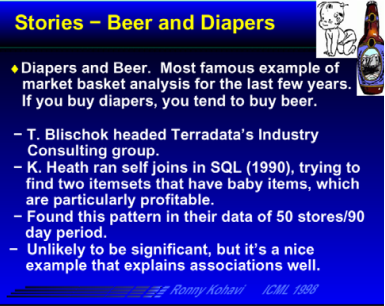
\includegraphics[scale=0.9]{images/lec08-pic02.png}
\end{figure}
\end{frame}

\begin{frame}{Как можно использовать ассоциативные правила?}
\begin{itemize}
\item пусть правило имеет вид
  \begin{figure}[h]
  \centering
  
\includegraphics[scale=0.9]{images/lec08-pic03.png}
  \end{figure}
\item "Potato chips": следствие - продажи чего мы собираемся (можем) увеличивать
\item "Bagels": антецедент - какие продукты будут влиять на продажу, если объявить скидки
\item "Bagels -> Potato chips": какие продукты следует размещать рядом, чтобы увеличить продажи "Potato Chips"
\end{itemize}
Практическое применение:
\begin{itemize}
\item оптимизировать размещение товара на полках
\item формировать персональные рекомендации
\item планирование промо-акции
\item более эффективно управлять ценами и ассортиментом
\end{itemize}
\end{frame}

\begin{frame}{Ассоциативные правила: основные понятия}
\begin{block}{Исходные данные}
  \begin{enumerate}
  \item база данных \textbf{транзакций}
  \item транзакция содержит список \textbf{элементов}
  \end{enumerate}
\end{block}
\begin{block}{Результаты поиска ассоциативных правил}
  \begin{enumerate}
  \item все правила, которые связывают наличие одного \textbf{набора}(itemset) с другим набором элементов
  \end{enumerate}
\end{block}
Например, $98\%$ людей, которые покупают шины и автоаксессуары, также заказывают услуги шионмонтажа.
\end{frame}

\begin{frame}{Ассоциативные правила: поддержка и значимость}
\[A \Rightarrow B [ s, c ]\]

\textbf{Поддержка (Support)}: обозначает, как часто правило встречается в транзакциях. 

\[support(A \Rightarrow B [ s, c ]) = p(A \cup B)\]

Значимость (confidence): обозначает процент транакций, содержащая \textbf{А}, которые содержат также \textbf{B}. Значимость - это оценка условной вероятности:

\[confidence(A \Rightarrow B [ s, c ]) = p(B|A) = sup(A,B)/sup(A)\]
\end{frame}

\begin{frame}{Пример}
\begin{figure}[h]
\centering
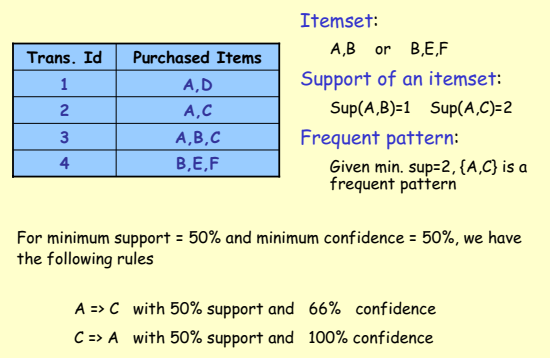
\includegraphics[scale=0.75]{images/lec08-pic04.png}
\end{figure}
\end{frame}

\begin{frame}{Математические обозначения}
\begin{figure}[h]
\centering
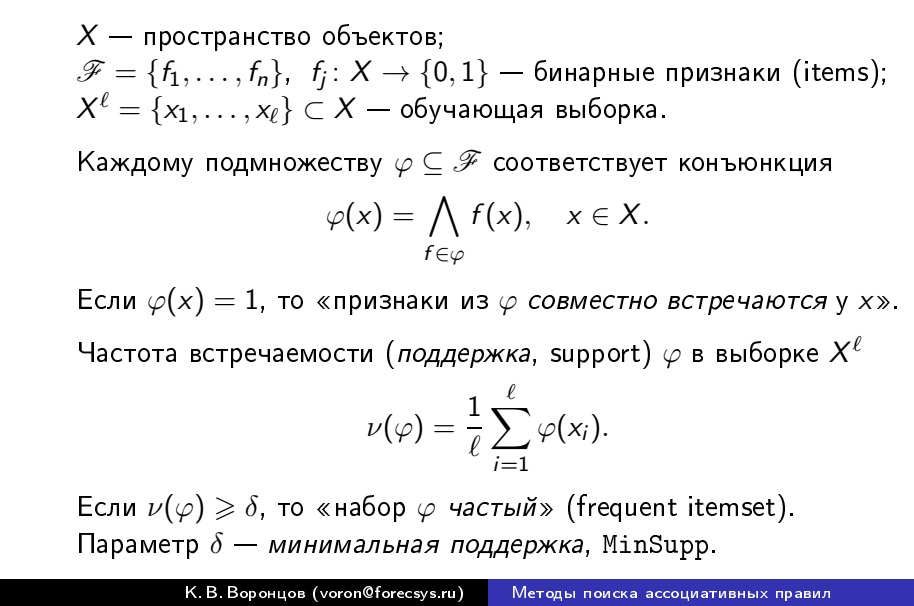
\includegraphics[scale=0.4]{images/lec08-pic05.png}
\end{figure}
\end{frame}

\begin{frame}{Математические обозначения}
\begin{figure}[h]
\centering
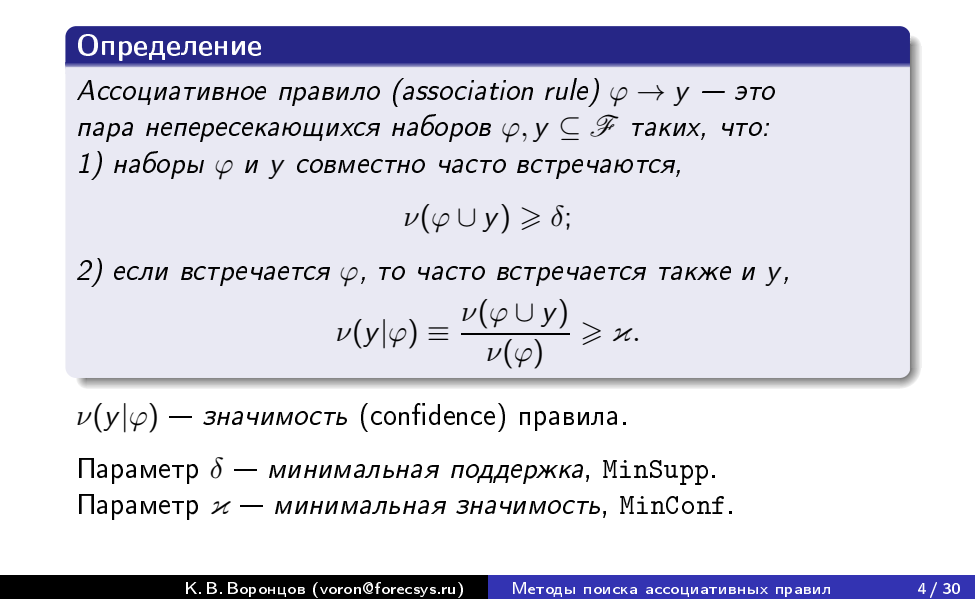
\includegraphics[scale=0.4]{images/lec08-pic06.png}
\end{figure}
\end{frame}

\section{Алгоритм поиска ассоциативных правил}
\begin{frame}{Логические (булевые) ассоциативные правила}
\begin{figure}[h]
\centering
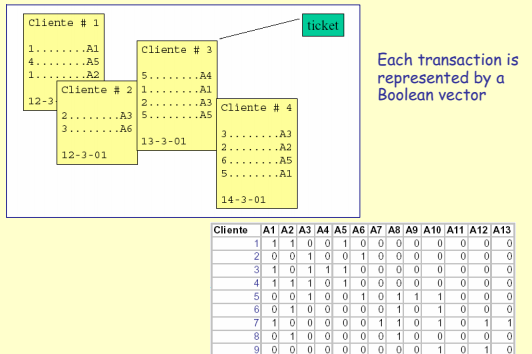
\includegraphics[scale=0.75]{images/lec08-pic07.png}
\end{figure}
\end{frame}

\begin{frame}{Пример поиска ассоциативных правил}
\begin{figure}[h]
\centering
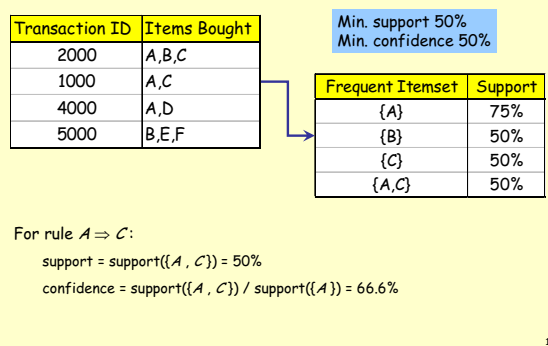
\includegraphics[scale=0.75]{images/lec08-pic08.png}
\end{figure}
\end{frame}

\begin{frame}{Принцип Apriori}
\begin{figure}[h]
\centering
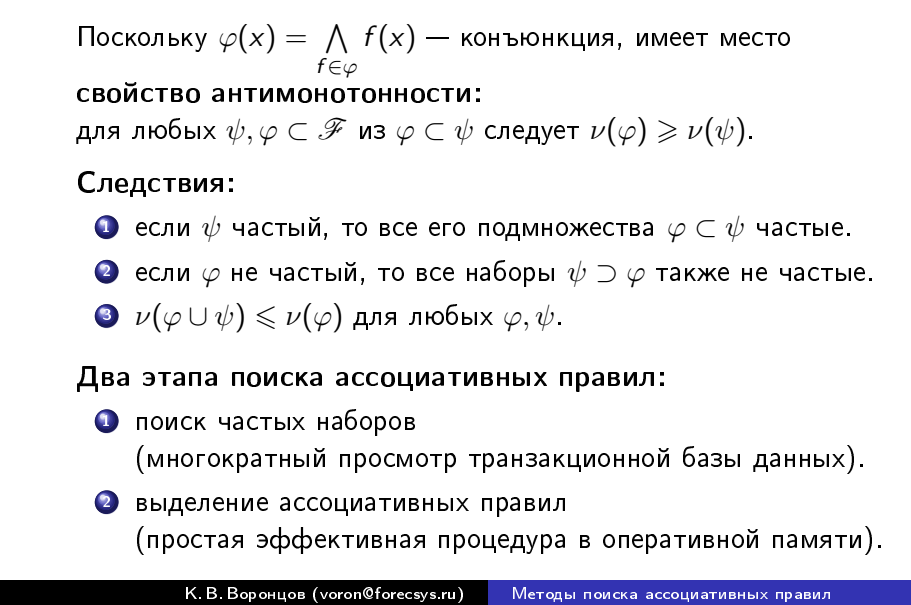
\includegraphics[scale=0.45]{images/lec08-pic09.png}
\end{figure}
\end{frame}

\begin{frame}{Принцип Apriori: множество наборов}
\begin{figure}[h]
\centering
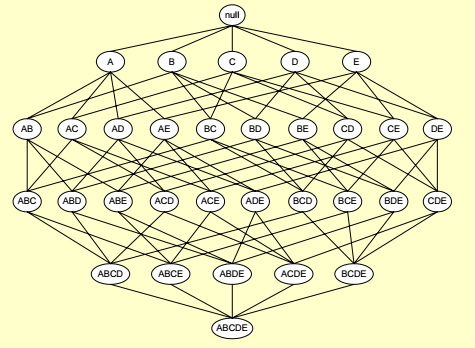
\includegraphics[scale=0.75]{images/lec08-pic10.png}
\end{figure}
\end{frame}

\begin{frame}{Принцип Apriori: не рассматриваемые наборы}
\begin{figure}[h]
\centering
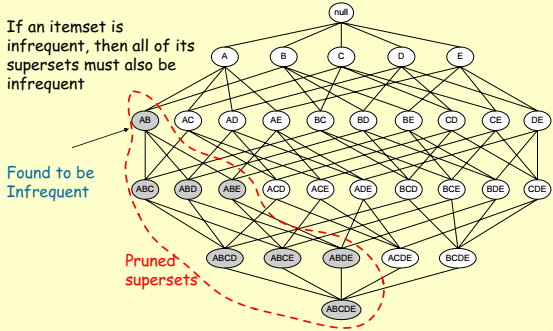
\includegraphics[scale=0.75]{images/lec08-pic11.png}
\end{figure}
\end{frame}

\begin{frame}{Принцип Apriori: основная идея - поиск в ширину}
\begin{figure}[h]
\centering
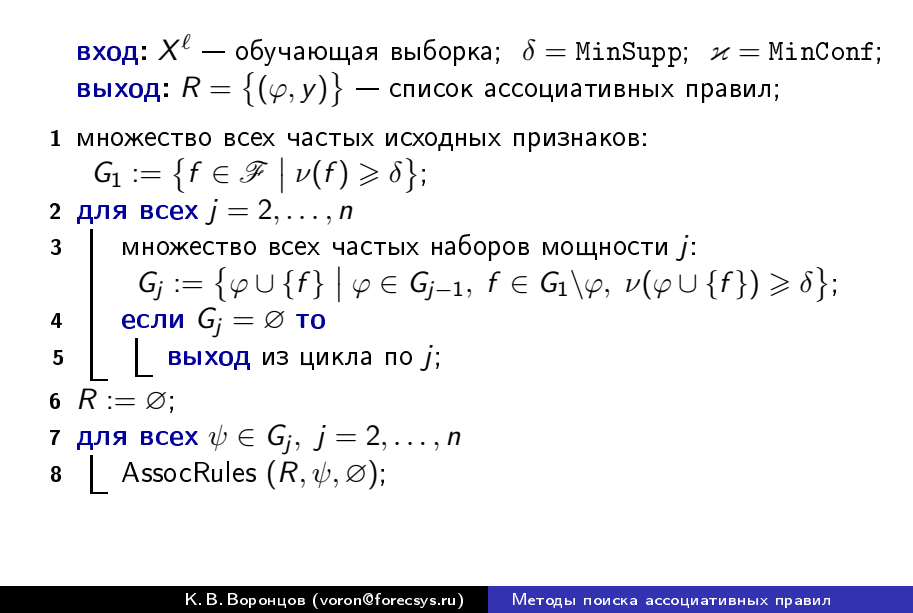
\includegraphics[scale=0.45]{images/lec08-pic12.png}
\end{figure}
\end{frame}

\begin{frame}{Принцип Apriori: пример}
\begin{figure}[h]
\centering
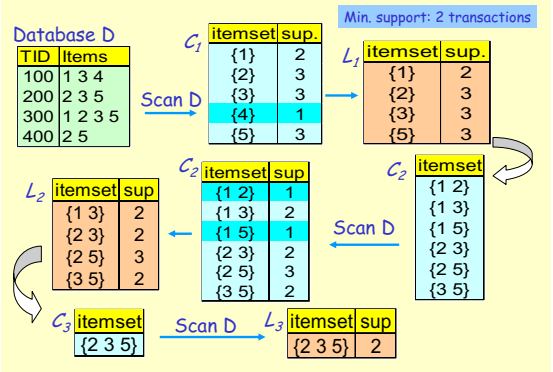
\includegraphics[scale=0.75]{images/lec08-pic13.png}
\end{figure}
\end{frame}

\begin{frame}{Принцип Apriori: пример}
\begin{figure}[h]
\centering
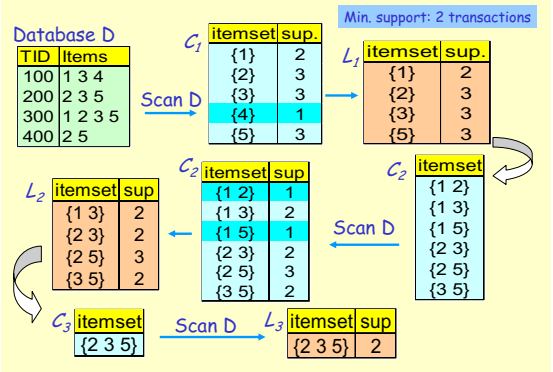
\includegraphics[scale=0.75]{images/lec08-pic13.png}
\end{figure}
\end{frame}

\begin{frame}{Принцип Apriori: получение ассоциативных правил}
\begin{figure}[h]
\centering
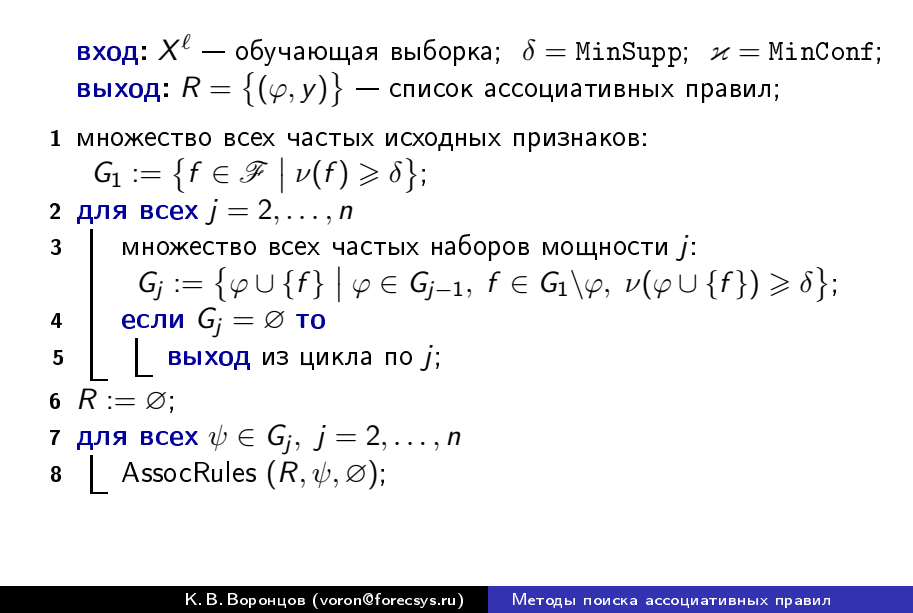
\includegraphics[scale=0.45]{images/lec08-pic12.png}
\end{figure}
\end{frame}

\begin{frame}{Выделение ассоциативных правил}
\[confidence(A\Rightarrow B)= P(B|A) = support(A\cup B)/support(A)\]

\begin{itemize}
\item Для каждого частого набора элементов x сгенерировать все непустые
подмножества x
\item Для каждого непустого подмножества x множества s получить правило:
\end{itemize}
\[s \Rightarrow (s\setminus x)\]
\[если\]
\[support(x)/support(s) > min_conf\]
\end{frame}

\begin{frame}{Выделение ассоциативных правил}
\begin{figure}[h]
\centering
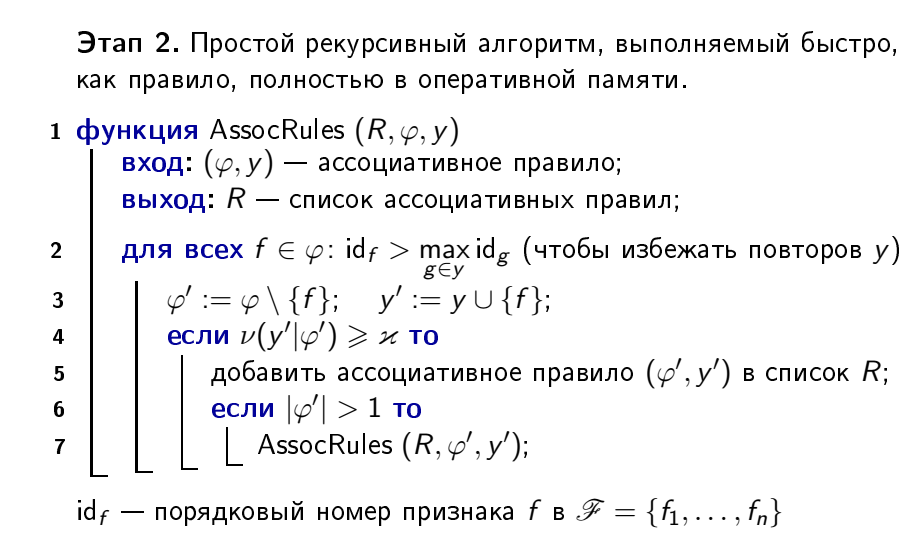
\includegraphics[scale=0.45]{images/lec08-pic14.png}
\end{figure}
\end{frame}

\begin{frame}{Пример}
Задан часто встречающийся набор (A, B, E). Какие возможны ассоциативные правила?
\begin{figure}[h]
\centering
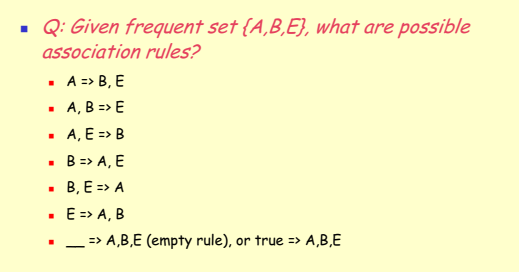
\includegraphics[scale=0.75]{images/lec08-pic15.png}
\end{figure}
\end{frame}

\begin{frame}{Пример}
\begin{figure}[h]
\centering
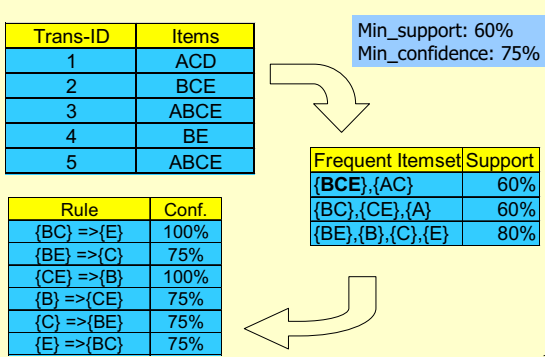
\includegraphics[scale=0.75]{images/lec08-pic16.png}
\end{figure}
\end{frame}

\begin{frame}{Упражнение}
\begin{figure}[h]
\centering
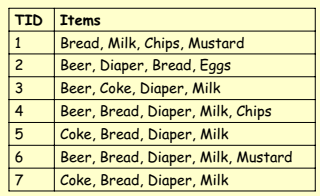
\includegraphics[scale=0.75]{images/lec08-pic17.png}
\end{figure}
\end{frame}

\begin{frame}{Упражнение}
\begin{figure}[h]
\centering
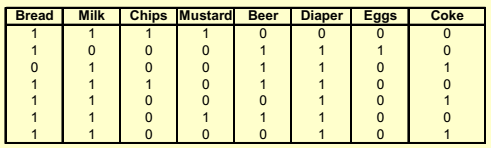
\includegraphics[scale=0.75]{images/lec08-pic18.png}
\end{figure}
\end{frame}

\begin{frame}{Упражнение}
\begin{figure}[h]
\centering
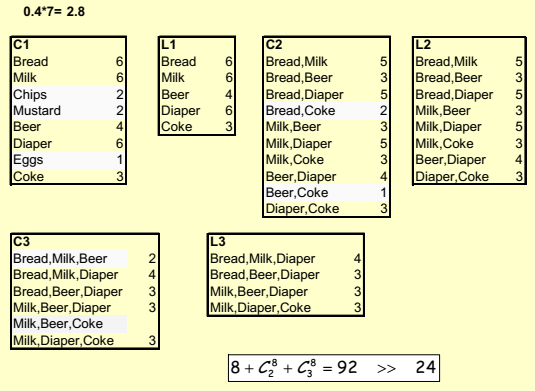
\includegraphics[scale=0.75]{images/lec08-pic19.png}
\end{figure}
\end{frame}

\begin{frame}{Модификация алгоритма Apriori}
Основные проблемы при генерации наборов:
\begin{itemize}
\item общее число транзакций может быть очень большим
\item одна транзакция может содержать много элементов
\end{itemize}
Модификации алгоритма:
\begin{itemize}
\item более эффективные структуры данных для быстрого поиска
\item поиск по частичной случайной выборке при пониженных поддержке и значимости с последующей проверкой на полной базе
\item алгоритмы, учитывающие иерархию признаков
\item поиск последовательных шаблонов
\item учет информации о клиентах
\end{itemize}
\end{frame}

\begin{frame}{Модификации алгоритма Apriori}
\begin{itemize}
\item \textbf{Проблема}: на каждом уровне осуществляется просмотр всей базы данных транзакций
\item AprioriTID: 
  \begin{itemize}
  \item генерировать набора как в алгоритме Аpriori, но БД используется для вычисления поддержки всех наборов за один проход;
  \item требуется значительно больше памяти;
  \item вычисляются и хранятся часто встречающиеся наборы $C\hat{\text{ }}_k$ для каждой транзакции;
  \end{itemize}
\item AprioriHybrid 
  \begin{itemize}
  \item на начальном этапе используется алгоритм Apriori;
  \item вычисляется размер $C\hat{\text{ }}_k$; 
  \item как только $C\hat{\text{ }}_k$ будет умещаться в памяти, переключиться на AprioriTid.
  \end{itemize}
\end{itemize}
\end{frame}

\begin{frame}{Пример}
\begin{figure}[h]
\centering
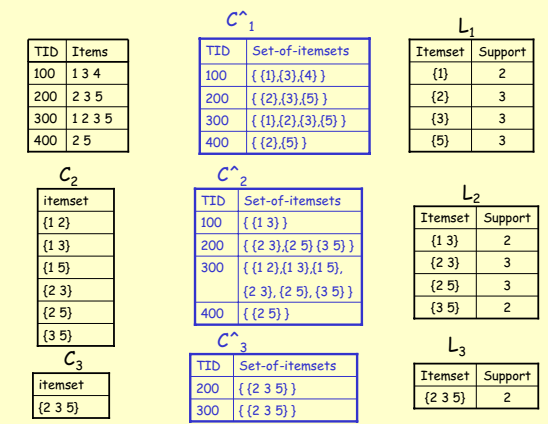
\includegraphics[scale=0.6]{images/lec08-pic20.png}
\end{figure}
\end{frame}

\begin{frame}{Какие правила интересны?}
\begin{itemize}
\item все ли найденные правила будут полезны и интересны?
\item как можно измерить "интересность" правила?
\end{itemize}
Субъективные критерии:
\begin{itemize}
\item правило интересно, если оно неожиданно для пользователя и/или полезно (пользователь может его применить)
\end{itemize}
Объективные критерии:
\begin{itemize}
\item поддержка (support)
\item значимость (confidence)
\item поддержка (Lift, Interest, Correlation) 
\item убедительность (Conviction)
\item влияние (Leverage, Piatetsky-Shapiro)
\item покрытие (Coverage)
\end{itemize}
\end{frame}

\begin{frame}{Пример}
\begin{figure}[h]
\centering
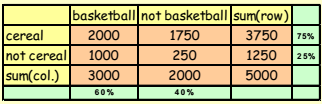
\includegraphics[scale=0.6]{images/lec08-pic21.png}
\end{figure}
\end{frame}

\begin{frame}{Пример}
\begin{figure}[h]
\centering
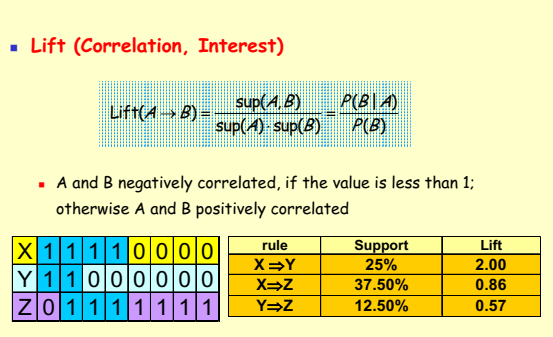
\includegraphics[scale=0.6]{images/lec08-pic22.png}
\end{figure}
\end{frame}

\begin{frame}{Пример}
\begin{figure}[h]
\centering
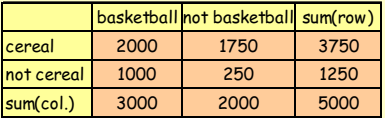
\includegraphics[scale=0.6]{images/lec08-pic23.png}
\end{figure}
\end{frame}

\begin{frame}{Пример}
\begin{figure}[h]
\centering
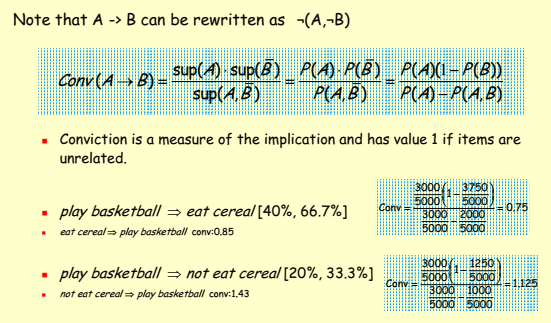
\includegraphics[scale=0.6]{images/lec08-pic24.png}
\end{figure}
\end{frame}

\begin{frame}{Пример}
\begin{figure}[h]
\centering
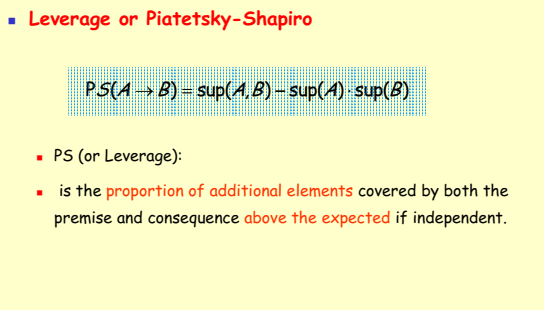
\includegraphics[scale=0.6]{images/lec08-pic25.png}
\end{figure}
\end{frame}

\begin{frame}{Пример}
\begin{figure}[h]
\centering
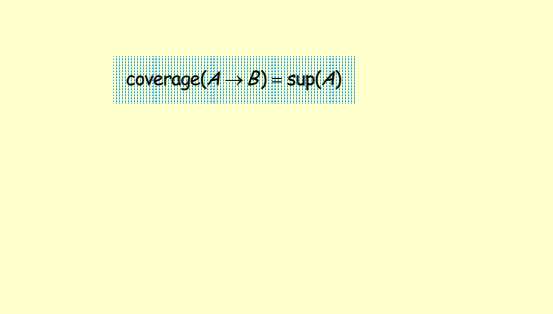
\includegraphics[scale=0.6]{images/lec08-pic26.png}
\end{figure}
\end{frame}

\begin{frame}{Пример}
\begin{figure}[h]
\centering
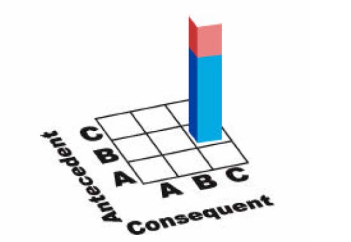
\includegraphics[scale=0.6]{images/lec08-pic27.png}
\end{figure}
\end{frame}

\end{document}